% !TeX root = ../../main.tex
\section{Kinetics}
\subsection{Nitration of toluene}
The nitrotoluene production has been started by reacting 95\% toluene and 70 \% nitric acid to produce 3 different nitrotoluene isomers of 4-ONT, 4-MNT and 4-PNT in a packed-bed reactor operating at 330K and X atm. 
%include Chemdraw here
\begin{scheme}[h]
    \centering
    \ch{ TOL + HNO3 -> ONT + MNT + PNT + H2O}
    \caption{Toluene nitration to nitrotoluene isomers}
    \label{eqn: nitration}
\end{scheme}
The rate equation can be defined as a first-order rate express

\begin{figure}[h]
    \centering
    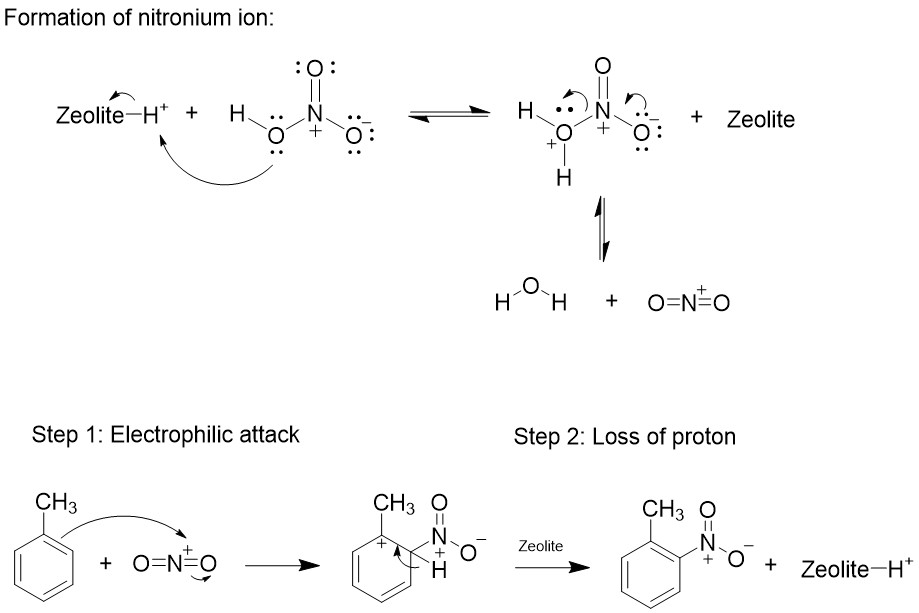
\includegraphics[width=\linewidth]{chapters/2-reaction/figures/Nitration.jpg}
    \caption{Mechanism for nitration of toluene}
    \label{fig:finalroutes}
\end{figure}

Brønsted acid sites on H-Mordenite 

\subsection{Hydrogenation of o-nitrotoluene}
After the production of the 3 nitrotoluene isomers, (mention separation?) ONT is mixed with propanol and hydrogenated to o-TOL in a co-current trickle bed reactor operating at 333K and 3 atm. 

\begin{scheme}[h]
    \centering
    \ch{ ONT + 3 H2 -> O{-}TOL + 2 H2O }
    \caption{ONT hydrogenation to O-TOL}
    \label{eqn: ONT hydrogenation}
\end{scheme}

include ChemDraw here
The rate equation for this equation can be defined as: 
\begin{equation}
    r = k P_{H_2}^{0.3} 
    \label{ONT rate equation}
\end{equation}
 \begin{equation}
     k = 211.69 exp(-\frac{45.52 \cdot 10^{3}}{RT} \frac{mol}{kPa^{0.3}g_{cat}s})
 \end{equation}
\subsection{Oxidation of p-nitrotoluene}
\subsection{Hydrogenation of nitrobenzaldehyde and nitrobenzoic acid}